\documentclass[1p]{elsarticle_modified}
%\bibliographystyle{elsarticle-num}

%\usepackage[colorlinks]{hyperref}
%\usepackage{abbrmath_seonhwa} %\Abb, \Ascr, \Acal ,\Abf, \Afrak
\usepackage{amsfonts}
\usepackage{amssymb}
\usepackage{amsmath}
\usepackage{amsthm}
\usepackage{scalefnt}
\usepackage{amsbsy}
\usepackage{kotex}
\usepackage{caption}
\usepackage{subfig}
\usepackage{color}
\usepackage{graphicx}
\usepackage{xcolor} %% white, black, red, green, blue, cyan, magenta, yellow
\usepackage{float}
\usepackage{setspace}
\usepackage{hyperref}

\usepackage{tikz}
\usetikzlibrary{arrows}

\usepackage{multirow}
\usepackage{array} % fixed length table
\usepackage{hhline}

%%%%%%%%%%%%%%%%%%%%%
\makeatletter
\renewcommand*\env@matrix[1][\arraystretch]{%
	\edef\arraystretch{#1}%
	\hskip -\arraycolsep
	\let\@ifnextchar\new@ifnextchar
	\array{*\c@MaxMatrixCols c}}
\makeatother %https://tex.stackexchange.com/questions/14071/how-can-i-increase-the-line-spacing-in-a-matrix
%%%%%%%%%%%%%%%

\usepackage[normalem]{ulem}

\newcommand{\msout}[1]{\ifmmode\text{\sout{\ensuremath{#1}}}\else\sout{#1}\fi}
%SOURCE: \msout is \stkout macro in https://tex.stackexchange.com/questions/20609/strikeout-in-math-mode

\newcommand{\cancel}[1]{
	\ifmmode
	{\color{red}\msout{#1}}
	\else
	{\color{red}\sout{#1}}
	\fi
}

\newcommand{\add}[1]{
	{\color{blue}\uwave{#1}}
}

\newcommand{\replace}[2]{
	\ifmmode
	{\color{red}\msout{#1}}{\color{blue}\uwave{#2}}
	\else
	{\color{red}\sout{#1}}{\color{blue}\uwave{#2}}
	\fi
}

\newcommand{\Sol}{\mathcal{S}} %segment
\newcommand{\D}{D} %diagram
\newcommand{\A}{\mathcal{A}} %arc


%%%%%%%%%%%%%%%%%%%%%%%%%%%%%5 test

\def\sl{\operatorname{\textup{SL}}(2,\Cbb)}
\def\psl{\operatorname{\textup{PSL}}(2,\Cbb)}
\def\quan{\mkern 1mu \triangleright \mkern 1mu}

\theoremstyle{definition}
\newtheorem{thm}{Theorem}[section]
\newtheorem{prop}[thm]{Proposition}
\newtheorem{lem}[thm]{Lemma}
\newtheorem{ques}[thm]{Question}
\newtheorem{cor}[thm]{Corollary}
\newtheorem{defn}[thm]{Definition}
\newtheorem{exam}[thm]{Example}
\newtheorem{rmk}[thm]{Remark}
\newtheorem{alg}[thm]{Algorithm}

\newcommand{\I}{\sqrt{-1}}
\begin{document}

%\begin{frontmatter}
%
%\title{Boundary parabolic representations of knots up to 8 crossings}
%
%%% Group authors per affiliation:
%\author{Yunhi Cho} 
%\address{Department of Mathematics, University of Seoul, Seoul, Korea}
%\ead{yhcho@uos.ac.kr}
%
%
%\author{Seonhwa Kim} %\fnref{s_kim}}
%\address{Center for Geometry and Physics, Institute for Basic Science, Pohang, 37673, Korea}
%\ead{ryeona17@ibs.re.kr}
%
%\author{Hyuk Kim}
%\address{Department of Mathematical Sciences, Seoul National University, Seoul 08826, Korea}
%\ead{hyukkim@snu.ac.kr}
%
%\author{Seokbeom Yoon}
%\address{Department of Mathematical Sciences, Seoul National University, Seoul, 08826,  Korea}
%\ead{sbyoon15@snu.ac.kr}
%
%\begin{abstract}
%We find all boundary parabolic representation of knots up to 8 crossings.
%
%\end{abstract}
%\begin{keyword}
%    \MSC[2010] 57M25 
%\end{keyword}
%
%\end{frontmatter}

%\linenumbers
%\tableofcontents
%
\newcommand\colored[1]{\textcolor{white}{\rule[-0.35ex]{0.8em}{1.4ex}}\kern-0.8em\color{red} #1}%
%\newcommand\colored[1]{\textcolor{white}{ #1}\kern-2.17ex	\textcolor{white}{ #1}\kern-1.81ex	\textcolor{white}{ #1}\kern-2.15ex\color{red}#1	}

{\Large $\underline{12a_{0025}~(K12a_{0025})}$}

\setlength{\tabcolsep}{10pt}
\renewcommand{\arraystretch}{1.6}
\vspace{1cm}\begin{tabular}{m{100pt}>{\centering\arraybackslash}m{274pt}}
\multirow{5}{120pt}{
	\centering
	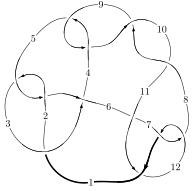
\includegraphics[width=112pt]{../../../GIT/diagram.site/Diagrams/png/826_12a_0025.png}\\
\ \ \ A knot diagram\footnotemark}&
\allowdisplaybreaks
\textbf{Linearized knot diagam} \\
\cline{2-2}
 &
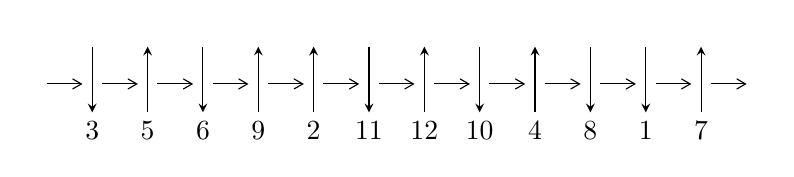
\begin{tikzpicture}[x=20pt, y=17pt]
	% nodes
	\node (C0) at (0, 0) {};
	\node (C1) at (1, 0) {};
	\node (C1U) at (1, +1) {};
	\node (C1D) at (1, -1) {3};

	\node (C2) at (2, 0) {};
	\node (C2U) at (2, +1) {};
	\node (C2D) at (2, -1) {5};

	\node (C3) at (3, 0) {};
	\node (C3U) at (3, +1) {};
	\node (C3D) at (3, -1) {6};

	\node (C4) at (4, 0) {};
	\node (C4U) at (4, +1) {};
	\node (C4D) at (4, -1) {9};

	\node (C5) at (5, 0) {};
	\node (C5U) at (5, +1) {};
	\node (C5D) at (5, -1) {2};

	\node (C6) at (6, 0) {};
	\node (C6U) at (6, +1) {};
	\node (C6D) at (6, -1) {11};

	\node (C7) at (7, 0) {};
	\node (C7U) at (7, +1) {};
	\node (C7D) at (7, -1) {12};

	\node (C8) at (8, 0) {};
	\node (C8U) at (8, +1) {};
	\node (C8D) at (8, -1) {10};

	\node (C9) at (9, 0) {};
	\node (C9U) at (9, +1) {};
	\node (C9D) at (9, -1) {4};

	\node (C10) at (10, 0) {};
	\node (C10U) at (10, +1) {};
	\node (C10D) at (10, -1) {8};

	\node (C11) at (11, 0) {};
	\node (C11U) at (11, +1) {};
	\node (C11D) at (11, -1) {1};

	\node (C12) at (12, 0) {};
	\node (C12U) at (12, +1) {};
	\node (C12D) at (12, -1) {7};
	\node (C13) at (13, 0) {};

	% arrows
	\draw[->,>={angle 60}]
	(C0) edge (C1) (C1) edge (C2) (C2) edge (C3) (C3) edge (C4) (C4) edge (C5) (C5) edge (C6) (C6) edge (C7) (C7) edge (C8) (C8) edge (C9) (C9) edge (C10) (C10) edge (C11) (C11) edge (C12) (C12) edge (C13) ;	\draw[->,>=stealth]
	(C1U) edge (C1D) (C2D) edge (C2U) (C3U) edge (C3D) (C4D) edge (C4U) (C5D) edge (C5U) (C6U) edge (C6D) (C7D) edge (C7U) (C8U) edge (C8D) (C9D) edge (C9U) (C10U) edge (C10D) (C11U) edge (C11D) (C12D) edge (C12U) ;
	\end{tikzpicture} \\
\hhline{~~} \\& 
\textbf{Solving Sequence} \\ \cline{2-2} 
 &
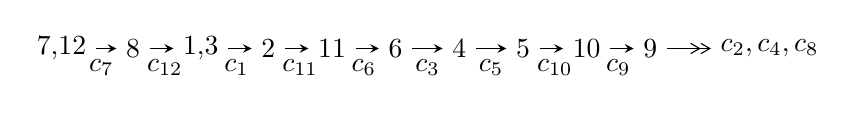
\begin{tikzpicture}[x=23pt, y=7pt]
	% node
	\node (A0) at (-1/8, 0) {7,12};
	\node (A1) at (1, 0) {8};
	\node (A2) at (33/16, 0) {1,3};
	\node (A3) at (25/8, 0) {2};
	\node (A4) at (33/8, 0) {11};
	\node (A5) at (41/8, 0) {6};
	\node (A6) at (49/8, 0) {4};
	\node (A7) at (57/8, 0) {5};
	\node (A8) at (65/8, 0) {10};
	\node (A9) at (73/8, 0) {9};
	\node (C1) at (1/2, -1) {$c_{7}$};
	\node (C2) at (3/2, -1) {$c_{12}$};
	\node (C3) at (21/8, -1) {$c_{1}$};
	\node (C4) at (29/8, -1) {$c_{11}$};
	\node (C5) at (37/8, -1) {$c_{6}$};
	\node (C6) at (45/8, -1) {$c_{3}$};
	\node (C7) at (53/8, -1) {$c_{5}$};
	\node (C8) at (61/8, -1) {$c_{10}$};
	\node (C9) at (69/8, -1) {$c_{9}$};
	\node (A10) at (11, 0) {$c_{2},c_{4},c_{8}$};

	% edge
	\draw[->,>=stealth]	
	(A0) edge (A1) (A1) edge (A2) (A2) edge (A3) (A3) edge (A4) (A4) edge (A5) (A5) edge (A6) (A6) edge (A7) (A7) edge (A8) (A8) edge (A9) ;
	\draw[->>,>={angle 60}]	
	(A9) edge (A10);
\end{tikzpicture} \\ 

\end{tabular} \\

\footnotetext{
The image of knot diagram is generated by the software ``\textbf{Draw programme}" developed by Andrew Bartholomew(\url{http://www.layer8.co.uk/maths/draw/index.htm\#Running-draw}), where we modified some parts for our purpose(\url{https://github.com/CATsTAILs/LinksPainter}).
}\phantom \\ \newline 
\centering \textbf{Ideals for irreducible components\footnotemark of $X_{\text{par}}$} 
 
\begin{align*}
I^u_{1}&=\langle 
u^{19}- u^{18}+\cdots- u^2+b,\;u^{19}- u^{18}+\cdots+a- u,\;u^{22}- u^{21}+\cdots- u+1\rangle \\
I^u_{2}&=\langle 
u^{73}-3 u^{72}+\cdots+b-2,\;-2 u^{72}-30 u^{70}+\cdots+a- u,\;u^{74}-2 u^{73}+\cdots-3 u+1\rangle \\
I^u_{3}&=\langle 
b+u+2,\;a+2,\;u^2+u+1\rangle \\
I^u_{4}&=\langle 
b-2 u-1,\;a-2 u-2,\;u^2+u+1\rangle \\
\\
\end{align*}
\raggedright * 4 irreducible components of $\dim_{\mathbb{C}}=0$, with total 100 representations.\\
\footnotetext{All coefficients of polynomials are rational numbers. But the coefficients are sometimes approximated in decimal forms when there is not enough margin.}
\newpage
\renewcommand{\arraystretch}{1}
\centering \section*{I. $I^u_{1}= \langle u^{19}- u^{18}+\cdots- u^2+b,\;u^{19}- u^{18}+\cdots+a- u,\;u^{22}- u^{21}+\cdots- u+1 \rangle$}
\flushleft \textbf{(i) Arc colorings}\\
\begin{tabular}{m{7pt} m{180pt} m{7pt} m{180pt} }
\flushright $a_{7}=$&$\begin{pmatrix}1\\0\end{pmatrix}$ \\
\flushright $a_{12}=$&$\begin{pmatrix}0\\u\end{pmatrix}$ \\
\flushright $a_{8}=$&$\begin{pmatrix}1\\- u^2\end{pmatrix}$ \\
\flushright $a_{1}=$&$\begin{pmatrix}u\\u\end{pmatrix}$ \\
\flushright $a_{3}=$&$\begin{pmatrix}- u^{19}+u^{18}+\cdots+u^2+u\\- u^{19}+u^{18}+\cdots-2 u^3+u^2\end{pmatrix}$ \\
\flushright $a_{2}=$&$\begin{pmatrix}u^{21}- u^{20}+\cdots- u^3+u\\u^{21}- u^{20}+\cdots- u^4+u\end{pmatrix}$ \\
\flushright $a_{11}=$&$\begin{pmatrix}u^3\\u^3+u\end{pmatrix}$ \\
\flushright $a_{6}=$&$\begin{pmatrix}- u^6- u^4+1\\- u^6-2 u^4- u^2\end{pmatrix}$ \\
\flushright $a_{4}=$&$\begin{pmatrix}- u^{19}+u^{18}+\cdots-3 u^3+u^2\\- u^{19}+u^{18}+\cdots- u^3+u^2\end{pmatrix}$ \\
\flushright $a_{5}=$&$\begin{pmatrix}- u^{20}+u^{19}+\cdots- u^2+u\\- u^{20}+u^{19}+\cdots+u-1\end{pmatrix}$ \\
\flushright $a_{10}=$&$\begin{pmatrix}u^5+2 u^3+u\\- u^7- u^5+u\end{pmatrix}$ \\
\flushright $a_{9}=$&$\begin{pmatrix}u^{10}+3 u^8+4 u^6+3 u^4+u^2+1\\- u^{12}-2 u^{10}-2 u^8+u^4\end{pmatrix}$\\&\end{tabular}
\flushleft \textbf{(ii) Obstruction class $= -1$}\\~\\
\flushleft \textbf{(iii) Cusp Shapes $= 4 u^{21}-8 u^{20}+26 u^{19}-42 u^{18}+82 u^{17}-116 u^{16}+164 u^{15}-198 u^{14}+226 u^{13}-232 u^{12}+234 u^{11}-206 u^{10}+198 u^9-168 u^8+152 u^7-132 u^6+100 u^5-72 u^4+50 u^3-18 u^2+14 u-6$}\\~\\
\newpage\renewcommand{\arraystretch}{1}
\flushleft \textbf{(iv) u-Polynomials at the component}\newline \\
\begin{tabular}{m{50pt}|m{274pt}}
Crossings & \hspace{64pt}u-Polynomials at each crossing \\
\hline $$\begin{aligned}c_{1},c_{11}\end{aligned}$$&$\begin{aligned}
&u^{22}+11 u^{21}+\cdots+3 u+1
\end{aligned}$\\
\hline $$\begin{aligned}c_{2},c_{5},c_{7}\\c_{12}\end{aligned}$$&$\begin{aligned}
&u^{22}+u^{21}+\cdots+u+1
\end{aligned}$\\
\hline $$\begin{aligned}c_{3},c_{6}\end{aligned}$$&$\begin{aligned}
&u^{22}- u^{21}+\cdots-3 u+1
\end{aligned}$\\
\hline $$\begin{aligned}c_{4},c_{9}\end{aligned}$$&$\begin{aligned}
&u^{22}+5 u^{21}+\cdots+8 u+4
\end{aligned}$\\
\hline $$\begin{aligned}c_{8},c_{10}\end{aligned}$$&$\begin{aligned}
&u^{22}+5 u^{21}+\cdots+56 u^2+16
\end{aligned}$\\
\hline
\end{tabular}\\~\\
\newpage\renewcommand{\arraystretch}{1}
\flushleft \textbf{(v) Riley Polynomials at the component}\newline \\
\begin{tabular}{m{50pt}|m{274pt}}
Crossings & \hspace{64pt}Riley Polynomials at each crossing \\
\hline $$\begin{aligned}c_{1},c_{11}\end{aligned}$$&$\begin{aligned}
&y^{22}+3 y^{21}+\cdots+11 y+1
\end{aligned}$\\
\hline $$\begin{aligned}c_{2},c_{5},c_{7}\\c_{12}\end{aligned}$$&$\begin{aligned}
&y^{22}+11 y^{21}+\cdots+3 y+1
\end{aligned}$\\
\hline $$\begin{aligned}c_{3},c_{6}\end{aligned}$$&$\begin{aligned}
&y^{22}-5 y^{21}+\cdots-13 y+1
\end{aligned}$\\
\hline $$\begin{aligned}c_{4},c_{9}\end{aligned}$$&$\begin{aligned}
&y^{22}+5 y^{21}+\cdots+56 y^2+16
\end{aligned}$\\
\hline $$\begin{aligned}c_{8},c_{10}\end{aligned}$$&$\begin{aligned}
&y^{22}+17 y^{21}+\cdots+1792 y+256
\end{aligned}$\\
\hline
\end{tabular}\\~\\
\newpage\flushleft \textbf{(vi) Complex Volumes and Cusp Shapes}
$$\begin{array}{c|c|c}  
\text{Solutions to }I^u_{1}& \I (\text{vol} + \sqrt{-1}CS) & \text{Cusp shape}\\
 \hline 
\begin{aligned}
u &= -0.267420 + 0.934374 I \\
a &= \phantom{-}0.866808 + 0.905520 I \\
b &= \phantom{-}1.134230 - 0.028854 I\end{aligned}
 & -2.03960 - 2.30169 I & -5.11682 + 3.55862 I \\ \hline\begin{aligned}
u &= -0.267420 - 0.934374 I \\
a &= \phantom{-}0.866808 - 0.905520 I \\
b &= \phantom{-}1.134230 + 0.028854 I\end{aligned}
 & -2.03960 + 2.30169 I & -5.11682 - 3.55862 I \\ \hline\begin{aligned}
u &= \phantom{-}0.803411 + 0.448160 I \\
a &= \phantom{-}1.64165 - 0.62510 I \\
b &= \phantom{-}0.838235 - 1.073260 I\end{aligned}
 & \phantom{-}6.81231 - 6.24031 I & \phantom{-}5.35592 + 2.94857 I \\ \hline\begin{aligned}
u &= \phantom{-}0.803411 - 0.448160 I \\
a &= \phantom{-}1.64165 + 0.62510 I \\
b &= \phantom{-}0.838235 + 1.073260 I\end{aligned}
 & \phantom{-}6.81231 + 6.24031 I & \phantom{-}5.35592 - 2.94857 I \\ \hline\begin{aligned}
u &= -0.773574 + 0.483952 I \\
a &= -1.84656 - 0.54883 I \\
b &= -1.07298 - 1.03278 I\end{aligned}
 & \phantom{-}7.30323 - 0.05327 I & \phantom{-}6.29197 + 2.01808 I \\ \hline\begin{aligned}
u &= -0.773574 - 0.483952 I \\
a &= -1.84656 + 0.54883 I \\
b &= -1.07298 + 1.03278 I\end{aligned}
 & \phantom{-}7.30323 + 0.05327 I & \phantom{-}6.29197 - 2.01808 I \\ \hline\begin{aligned}
u &= \phantom{-}0.125921 + 1.085150 I \\
a &= \phantom{-}0.002278 + 0.829637 I \\
b &= -0.123644 - 0.255513 I\end{aligned}
 & -3.59209 - 2.19399 I & -7.43206 + 2.16700 I \\ \hline\begin{aligned}
u &= \phantom{-}0.125921 - 1.085150 I \\
a &= \phantom{-}0.002278 - 0.829637 I \\
b &= -0.123644 + 0.255513 I\end{aligned}
 & -3.59209 + 2.19399 I & -7.43206 - 2.16700 I \\ \hline\begin{aligned}
u &= -0.469571 + 1.049440 I \\
a &= -0.16005 - 2.27593 I \\
b &= \phantom{-}0.30952 - 3.32537 I\end{aligned}
 & -2.42559 - 6.55386 I & -3.45447 + 8.04873 I \\ \hline\begin{aligned}
u &= -0.469571 - 1.049440 I \\
a &= -0.16005 + 2.27593 I \\
b &= \phantom{-}0.30952 + 3.32537 I\end{aligned}
 & -2.42559 + 6.55386 I & -3.45447 - 8.04873 I\\
 \hline 
 \end{array}$$\newpage$$\begin{array}{c|c|c}  
\text{Solutions to }I^u_{1}& \I (\text{vol} + \sqrt{-1}CS) & \text{Cusp shape}\\
 \hline 
\begin{aligned}
u &= \phantom{-}0.361702 + 1.107050 I \\
a &= \phantom{-}0.209067 - 0.490062 I \\
b &= -0.15263 - 1.59711 I\end{aligned}
 & -7.56344 + 3.87204 I & -10.26851 - 4.35879 I \\ \hline\begin{aligned}
u &= \phantom{-}0.361702 - 1.107050 I \\
a &= \phantom{-}0.209067 + 0.490062 I \\
b &= -0.15263 + 1.59711 I\end{aligned}
 & -7.56344 - 3.87204 I & -10.26851 + 4.35879 I \\ \hline\begin{aligned}
u &= \phantom{-}0.510802 + 1.115330 I \\
a &= \phantom{-}1.37025 - 1.89407 I \\
b &= \phantom{-}0.85945 - 3.00940 I\end{aligned}
 & -5.48268 + 11.20780 I & -5.92791 - 10.64614 I \\ \hline\begin{aligned}
u &= \phantom{-}0.510802 - 1.115330 I \\
a &= \phantom{-}1.37025 + 1.89407 I \\
b &= \phantom{-}0.85945 + 3.00940 I\end{aligned}
 & -5.48268 - 11.20780 I & -5.92791 + 10.64614 I \\ \hline\begin{aligned}
u &= -0.611674 + 1.083050 I \\
a &= -2.45227 - 2.64694 I \\
b &= -1.84060 - 3.72999 I\end{aligned}
 & \phantom{-}3.70474 - 10.43210 I & \phantom{-}0.79280 + 7.46958 I \\ \hline\begin{aligned}
u &= -0.611674 - 1.083050 I \\
a &= -2.45227 + 2.64694 I \\
b &= -1.84060 + 3.72999 I\end{aligned}
 & \phantom{-}3.70474 + 10.43210 I & \phantom{-}0.79280 - 7.46958 I \\ \hline\begin{aligned}
u &= \phantom{-}0.620139 + 1.106350 I \\
a &= \phantom{-}2.54875 - 2.41058 I \\
b &= \phantom{-}1.92861 - 3.51693 I\end{aligned}
 & \phantom{-}2.8718 + 16.9388 I & -0.30393 - 11.38128 I \\ \hline\begin{aligned}
u &= \phantom{-}0.620139 - 1.106350 I \\
a &= \phantom{-}2.54875 + 2.41058 I \\
b &= \phantom{-}1.92861 + 3.51693 I\end{aligned}
 & \phantom{-}2.8718 - 16.9388 I & -0.30393 + 11.38128 I \\ \hline\begin{aligned}
u &= \phantom{-}0.619109 + 0.241097 I \\
a &= \phantom{-}1.096950 + 0.038223 I \\
b &= \phantom{-}0.477839 - 0.202874 I\end{aligned}
 & -0.59135 - 2.31883 I & \phantom{-}1.12676 + 3.72876 I \\ \hline\begin{aligned}
u &= \phantom{-}0.619109 - 0.241097 I \\
a &= \phantom{-}1.096950 - 0.038223 I \\
b &= \phantom{-}0.477839 + 0.202874 I\end{aligned}
 & -0.59135 + 2.31883 I & \phantom{-}1.12676 - 3.72876 I\\
 \hline 
 \end{array}$$\newpage$$\begin{array}{c|c|c}  
\text{Solutions to }I^u_{1}& \I (\text{vol} + \sqrt{-1}CS) & \text{Cusp shape}\\
 \hline 
\begin{aligned}
u &= -0.418845 + 0.499289 I \\
a &= -1.27687 + 1.05838 I \\
b &= -0.858029 + 0.559094 I\end{aligned}
 & \phantom{-}1.00269 - 1.14066 I & \phantom{-}4.93625 + 3.17573 I \\ \hline\begin{aligned}
u &= -0.418845 - 0.499289 I \\
a &= -1.27687 - 1.05838 I \\
b &= -0.858029 - 0.559094 I\end{aligned}
 & \phantom{-}1.00269 + 1.14066 I & \phantom{-}4.93625 - 3.17573 I\\
 \hline 
 \end{array}$$\newpage\newpage\renewcommand{\arraystretch}{1}
\centering \section*{II. $I^u_{2}= \langle u^{73}-3 u^{72}+\cdots+b-2,\;-2 u^{72}-30 u^{70}+\cdots+a- u,\;u^{74}-2 u^{73}+\cdots-3 u+1 \rangle$}
\flushleft \textbf{(i) Arc colorings}\\
\begin{tabular}{m{7pt} m{180pt} m{7pt} m{180pt} }
\flushright $a_{7}=$&$\begin{pmatrix}1\\0\end{pmatrix}$ \\
\flushright $a_{12}=$&$\begin{pmatrix}0\\u\end{pmatrix}$ \\
\flushright $a_{8}=$&$\begin{pmatrix}1\\- u^2\end{pmatrix}$ \\
\flushright $a_{1}=$&$\begin{pmatrix}u\\u\end{pmatrix}$ \\
\flushright $a_{3}=$&$\begin{pmatrix}2 u^{72}+30 u^{70}+\cdots+2 u^2+u\\- u^{73}+3 u^{72}+\cdots-2 u+2\end{pmatrix}$ \\
\flushright $a_{2}=$&$\begin{pmatrix}2 u^{72}-2 u^{71}+\cdots-6 u+3\\- u^{73}+3 u^{72}+\cdots-5 u+2\end{pmatrix}$ \\
\flushright $a_{11}=$&$\begin{pmatrix}u^3\\u^3+u\end{pmatrix}$ \\
\flushright $a_{6}=$&$\begin{pmatrix}- u^6- u^4+1\\- u^6-2 u^4- u^2\end{pmatrix}$ \\
\flushright $a_{4}=$&$\begin{pmatrix}-2 u^{73}+3 u^{72}+\cdots- u-1\\- u^{73}-13 u^{71}+\cdots+3 u-1\end{pmatrix}$ \\
\flushright $a_{5}=$&$\begin{pmatrix}- u^{72}- u^{71}+\cdots- u+1\\u^{73}-2 u^{72}+\cdots+u-1\end{pmatrix}$ \\
\flushright $a_{10}=$&$\begin{pmatrix}u^5+2 u^3+u\\- u^7- u^5+u\end{pmatrix}$ \\
\flushright $a_{9}=$&$\begin{pmatrix}u^{10}+3 u^8+4 u^6+3 u^4+u^2+1\\- u^{12}-2 u^{10}-2 u^8+u^4\end{pmatrix}$\\&\end{tabular}
\flushleft \textbf{(ii) Obstruction class $= -1$}\\~\\
\flushleft \textbf{(iii) Cusp Shapes $= -3 u^{73}+8 u^{72}+\cdots-7 u+7$}\\~\\
\newpage\renewcommand{\arraystretch}{1}
\flushleft \textbf{(iv) u-Polynomials at the component}\newline \\
\begin{tabular}{m{50pt}|m{274pt}}
Crossings & \hspace{64pt}u-Polynomials at each crossing \\
\hline $$\begin{aligned}c_{1},c_{11}\end{aligned}$$&$\begin{aligned}
&u^{74}+32 u^{73}+\cdots+5 u+1
\end{aligned}$\\
\hline $$\begin{aligned}c_{2},c_{5},c_{7}\\c_{12}\end{aligned}$$&$\begin{aligned}
&u^{74}+2 u^{73}+\cdots+3 u+1
\end{aligned}$\\
\hline $$\begin{aligned}c_{3},c_{6}\end{aligned}$$&$\begin{aligned}
&u^{74}-2 u^{73}+\cdots-3 u+1
\end{aligned}$\\
\hline $$\begin{aligned}c_{4},c_{9}\end{aligned}$$&$\begin{aligned}
&(u^{37}-2 u^{36}+\cdots- u-2)^{2}
\end{aligned}$\\
\hline $$\begin{aligned}c_{8},c_{10}\end{aligned}$$&$\begin{aligned}
&(u^{37}+10 u^{36}+\cdots-39 u-4)^{2}
\end{aligned}$\\
\hline
\end{tabular}\\~\\
\newpage\renewcommand{\arraystretch}{1}
\flushleft \textbf{(v) Riley Polynomials at the component}\newline \\
\begin{tabular}{m{50pt}|m{274pt}}
Crossings & \hspace{64pt}Riley Polynomials at each crossing \\
\hline $$\begin{aligned}c_{1},c_{11}\end{aligned}$$&$\begin{aligned}
&y^{74}+20 y^{73}+\cdots+37 y+1
\end{aligned}$\\
\hline $$\begin{aligned}c_{2},c_{5},c_{7}\\c_{12}\end{aligned}$$&$\begin{aligned}
&y^{74}+32 y^{73}+\cdots+5 y+1
\end{aligned}$\\
\hline $$\begin{aligned}c_{3},c_{6}\end{aligned}$$&$\begin{aligned}
&y^{74}+8 y^{73}+\cdots+101 y+1
\end{aligned}$\\
\hline $$\begin{aligned}c_{4},c_{9}\end{aligned}$$&$\begin{aligned}
&(y^{37}+10 y^{36}+\cdots-39 y-4)^{2}
\end{aligned}$\\
\hline $$\begin{aligned}c_{8},c_{10}\end{aligned}$$&$\begin{aligned}
&(y^{37}+34 y^{36}+\cdots-159 y-16)^{2}
\end{aligned}$\\
\hline
\end{tabular}\\~\\
\newpage\flushleft \textbf{(vi) Complex Volumes and Cusp Shapes}
$$\begin{array}{c|c|c}  
\text{Solutions to }I^u_{2}& \I (\text{vol} + \sqrt{-1}CS) & \text{Cusp shape}\\
 \hline 
\begin{aligned}
u &= -0.639479 + 0.752607 I \\
a &= -2.15983 + 0.09363 I \\
b &= -1.93455 - 1.15641 I\end{aligned}
 & -0.61107 - 5.41655 I & \phantom{-0.000000 -}0. + 9.62417 I \\ \hline\begin{aligned}
u &= -0.639479 - 0.752607 I \\
a &= -2.15983 - 0.09363 I \\
b &= -1.93455 + 1.15641 I\end{aligned}
 & -0.61107 + 5.41655 I & \phantom{-0.000000 } 0. - 9.62417 I \\ \hline\begin{aligned}
u &= -0.784429 + 0.545941 I \\
a &= -2.03595 - 0.33437 I \\
b &= -1.91239 - 1.94292 I\end{aligned}
 & \phantom{-}5.47701 - 8.31264 I & \phantom{-}3.19623 + 7.51099 I \\ \hline\begin{aligned}
u &= -0.784429 - 0.545941 I \\
a &= -2.03595 + 0.33437 I \\
b &= -1.91239 + 1.94292 I\end{aligned}
 & \phantom{-}5.47701 + 8.31264 I & \phantom{-}3.19623 - 7.51099 I \\ \hline\begin{aligned}
u &= -0.047209 + 1.049760 I \\
a &= \phantom{-}2.14571 - 0.35342 I \\
b &= \phantom{-}0.925538 - 1.003280 I\end{aligned}
 & \phantom{-}0.33366 + 3.54390 I & \phantom{-0.000000 } 0 \\ \hline\begin{aligned}
u &= -0.047209 - 1.049760 I \\
a &= \phantom{-}2.14571 + 0.35342 I \\
b &= \phantom{-}0.925538 + 1.003280 I\end{aligned}
 & \phantom{-}0.33366 - 3.54390 I & \phantom{-0.000000 } 0 \\ \hline\begin{aligned}
u &= -0.779819 + 0.528531 I \\
a &= \phantom{-}0.740110 + 0.451946 I \\
b &= \phantom{-}0.62798 + 1.32561 I\end{aligned}
 & \phantom{-}7.26569 - 3.05590 I & \phantom{-}6.03502 + 2.77359 I \\ \hline\begin{aligned}
u &= -0.779819 - 0.528531 I \\
a &= \phantom{-}0.740110 - 0.451946 I \\
b &= \phantom{-}0.62798 - 1.32561 I\end{aligned}
 & \phantom{-}7.26569 + 3.05590 I & \phantom{-}6.03502 - 2.77359 I \\ \hline\begin{aligned}
u &= \phantom{-}0.009056 + 1.063140 I \\
a &= -1.19514 + 0.78248 I \\
b &= -0.491540 + 1.031220 I\end{aligned}
 & \phantom{-}1.91033 - 1.51255 I & \phantom{-0.000000 } 0 \\ \hline\begin{aligned}
u &= \phantom{-}0.009056 - 1.063140 I \\
a &= -1.19514 - 0.78248 I \\
b &= -0.491540 - 1.031220 I\end{aligned}
 & \phantom{-}1.91033 + 1.51255 I & \phantom{-0.000000 } 0\\
 \hline 
 \end{array}$$\newpage$$\begin{array}{c|c|c}  
\text{Solutions to }I^u_{2}& \I (\text{vol} + \sqrt{-1}CS) & \text{Cusp shape}\\
 \hline 
\begin{aligned}
u &= -0.622852 + 0.865244 I \\
a &= \phantom{-}0.79438 + 2.08172 I \\
b &= -0.29643 + 1.96964 I\end{aligned}
 & -0.936846 + 0.485539 I & \phantom{-0.000000 } 0 \\ \hline\begin{aligned}
u &= -0.622852 - 0.865244 I \\
a &= \phantom{-}0.79438 - 2.08172 I \\
b &= -0.29643 - 1.96964 I\end{aligned}
 & -0.936846 - 0.485539 I & \phantom{-0.000000 } 0 \\ \hline\begin{aligned}
u &= \phantom{-}0.813660 + 0.438643 I \\
a &= -2.38959 + 1.49627 I \\
b &= -0.90547 + 2.36932 I\end{aligned}
 & \phantom{-}4.86825 - 11.57530 I & \phantom{-}2.50814 + 7.25667 I \\ \hline\begin{aligned}
u &= \phantom{-}0.813660 - 0.438643 I \\
a &= -2.38959 - 1.49627 I \\
b &= -0.90547 - 2.36932 I\end{aligned}
 & \phantom{-}4.86825 + 11.57530 I & \phantom{-}2.50814 - 7.25667 I \\ \hline\begin{aligned}
u &= \phantom{-}0.443091 + 0.986263 I \\
a &= -1.38423 + 1.70607 I \\
b &= -0.33820 + 1.81029 I\end{aligned}
 & -0.936846 + 0.485539 I & \phantom{-0.000000 } 0 \\ \hline\begin{aligned}
u &= \phantom{-}0.443091 - 0.986263 I \\
a &= -1.38423 - 1.70607 I \\
b &= -0.33820 - 1.81029 I\end{aligned}
 & -0.936846 - 0.485539 I & \phantom{-0.000000 } 0 \\ \hline\begin{aligned}
u &= \phantom{-}0.775921 + 0.477218 I \\
a &= -0.740766 + 0.505518 I \\
b &= -0.57413 + 1.46540 I\end{aligned}
 & \phantom{-}7.26569 - 3.05590 I & \phantom{-}6.03502 + 2.77359 I \\ \hline\begin{aligned}
u &= \phantom{-}0.775921 - 0.477218 I \\
a &= -0.740766 - 0.505518 I \\
b &= -0.57413 - 1.46540 I\end{aligned}
 & \phantom{-}7.26569 + 3.05590 I & \phantom{-}6.03502 - 2.77359 I \\ \hline\begin{aligned}
u &= \phantom{-}0.762103 + 0.491833 I \\
a &= \phantom{-}1.87904 - 0.32585 I \\
b &= \phantom{-}1.73107 - 1.98585 I\end{aligned}
 & \phantom{-}5.70204 + 2.27936 I & \phantom{-}3.88815 - 2.05007 I \\ \hline\begin{aligned}
u &= \phantom{-}0.762103 - 0.491833 I \\
a &= \phantom{-}1.87904 + 0.32585 I \\
b &= \phantom{-}1.73107 + 1.98585 I\end{aligned}
 & \phantom{-}5.70204 - 2.27936 I & \phantom{-}3.88815 + 2.05007 I\\
 \hline 
 \end{array}$$\newpage$$\begin{array}{c|c|c}  
\text{Solutions to }I^u_{2}& \I (\text{vol} + \sqrt{-1}CS) & \text{Cusp shape}\\
 \hline 
\begin{aligned}
u &= -0.773218 + 0.464058 I \\
a &= \phantom{-}2.65308 + 1.45047 I \\
b &= \phantom{-}1.16242 + 2.27131 I\end{aligned}
 & \phantom{-}5.54616 + 5.20107 I & \phantom{-}3.66602 - 2.81386 I \\ \hline\begin{aligned}
u &= -0.773218 - 0.464058 I \\
a &= \phantom{-}2.65308 - 1.45047 I \\
b &= \phantom{-}1.16242 - 2.27131 I\end{aligned}
 & \phantom{-}5.54616 - 5.20107 I & \phantom{-}3.66602 + 2.81386 I \\ \hline\begin{aligned}
u &= -0.395925 + 1.024370 I \\
a &= -0.444820 - 1.150880 I \\
b &= -1.42676 - 1.64270 I\end{aligned}
 & -2.95124\phantom{ +0.000000I} & \phantom{-0.000000 } 0 \\ \hline\begin{aligned}
u &= -0.395925 - 1.024370 I \\
a &= -0.444820 + 1.150880 I \\
b &= -1.42676 + 1.64270 I\end{aligned}
 & -2.95124\phantom{ +0.000000I} & \phantom{-0.000000 } 0 \\ \hline\begin{aligned}
u &= -0.480742 + 0.988204 I \\
a &= -0.418583 + 1.307900 I \\
b &= -0.50569 + 1.47970 I\end{aligned}
 & -0.32230 - 2.77484 I & \phantom{-0.000000 } 0 \\ \hline\begin{aligned}
u &= -0.480742 - 0.988204 I \\
a &= -0.418583 - 1.307900 I \\
b &= -0.50569 - 1.47970 I\end{aligned}
 & -0.32230 + 2.77484 I & \phantom{-0.000000 } 0 \\ \hline\begin{aligned}
u &= -0.569891 + 0.939876 I \\
a &= -1.55469 + 0.28140 I \\
b &= -1.41271 - 0.18656 I\end{aligned}
 & \phantom{-}0.15880 - 2.93389 I & \phantom{-0.000000 } 0 \\ \hline\begin{aligned}
u &= -0.569891 - 0.939876 I \\
a &= -1.55469 - 0.28140 I \\
b &= -1.41271 + 0.18656 I\end{aligned}
 & \phantom{-}0.15880 + 2.93389 I & \phantom{-0.000000 } 0 \\ \hline\begin{aligned}
u &= -0.725089 + 0.517371 I \\
a &= -0.05378 + 1.70419 I \\
b &= -1.09918 + 0.98483 I\end{aligned}
 & \phantom{-}1.91033 - 1.51255 I & \phantom{-0.000000 -}0. + 2.66920 I \\ \hline\begin{aligned}
u &= -0.725089 - 0.517371 I \\
a &= -0.05378 - 1.70419 I \\
b &= -1.09918 - 0.98483 I\end{aligned}
 & \phantom{-}1.91033 + 1.51255 I & \phantom{-0.000000 } 0. - 2.66920 I\\
 \hline 
 \end{array}$$\newpage$$\begin{array}{c|c|c}  
\text{Solutions to }I^u_{2}& \I (\text{vol} + \sqrt{-1}CS) & \text{Cusp shape}\\
 \hline 
\begin{aligned}
u &= \phantom{-}0.324310 + 1.067530 I \\
a &= \phantom{-}0.368103 + 0.746898 I \\
b &= \phantom{-}0.134333 + 1.055790 I\end{aligned}
 & -4.13208 + 0.49053 I & \phantom{-0.000000 } 0 \\ \hline\begin{aligned}
u &= \phantom{-}0.324310 - 1.067530 I \\
a &= \phantom{-}0.368103 - 0.746898 I \\
b &= \phantom{-}0.134333 - 1.055790 I\end{aligned}
 & -4.13208 - 0.49053 I & \phantom{-0.000000 } 0 \\ \hline\begin{aligned}
u &= \phantom{-}0.771853 + 0.430210 I \\
a &= \phantom{-}0.12391 + 1.52352 I \\
b &= \phantom{-}1.27111 + 0.67805 I\end{aligned}
 & \phantom{-}1.41199 - 4.22774 I & -0.66777 + 2.80088 I \\ \hline\begin{aligned}
u &= \phantom{-}0.771853 - 0.430210 I \\
a &= \phantom{-}0.12391 - 1.52352 I \\
b &= \phantom{-}1.27111 - 0.67805 I\end{aligned}
 & \phantom{-}1.41199 + 4.22774 I & -0.66777 - 2.80088 I \\ \hline\begin{aligned}
u &= \phantom{-}0.478382 + 1.012710 I \\
a &= \phantom{-}1.86046 - 0.41541 I \\
b &= \phantom{-}1.14344 - 0.90963 I\end{aligned}
 & -0.61107 + 5.41655 I & \phantom{-0.000000 } 0 \\ \hline\begin{aligned}
u &= \phantom{-}0.478382 - 1.012710 I \\
a &= \phantom{-}1.86046 + 0.41541 I \\
b &= \phantom{-}1.14344 + 0.90963 I\end{aligned}
 & -0.61107 - 5.41655 I & \phantom{-0.000000 } 0 \\ \hline\begin{aligned}
u &= \phantom{-}0.071006 + 1.119930 I \\
a &= \phantom{-}1.061640 + 0.567159 I \\
b &= \phantom{-}0.447863 + 0.894942 I\end{aligned}
 & \phantom{-}1.41199 - 4.22774 I & \phantom{-0.000000 } 0 \\ \hline\begin{aligned}
u &= \phantom{-}0.071006 - 1.119930 I \\
a &= \phantom{-}1.061640 - 0.567159 I \\
b &= \phantom{-}0.447863 - 0.894942 I\end{aligned}
 & \phantom{-}1.41199 + 4.22774 I & \phantom{-0.000000 } 0 \\ \hline\begin{aligned}
u &= -0.552065 + 0.679047 I \\
a &= \phantom{-}0.318468 + 0.837668 I \\
b &= -0.026831 + 1.040650 I\end{aligned}
 & \phantom{-}0.94543 - 1.58284 I & \phantom{-}3.46208 + 5.25506 I \\ \hline\begin{aligned}
u &= -0.552065 - 0.679047 I \\
a &= \phantom{-}0.318468 - 0.837668 I \\
b &= -0.026831 - 1.040650 I\end{aligned}
 & \phantom{-}0.94543 + 1.58284 I & \phantom{-}3.46208 - 5.25506 I\\
 \hline 
 \end{array}$$\newpage$$\begin{array}{c|c|c}  
\text{Solutions to }I^u_{2}& \I (\text{vol} + \sqrt{-1}CS) & \text{Cusp shape}\\
 \hline 
\begin{aligned}
u &= \phantom{-}0.083389 + 1.139640 I \\
a &= -2.01039 - 0.09832 I \\
b &= -0.804300 - 0.746868 I\end{aligned}
 & -0.56297 - 9.41729 I & \phantom{-0.000000 } 0 \\ \hline\begin{aligned}
u &= \phantom{-}0.083389 - 1.139640 I \\
a &= -2.01039 + 0.09832 I \\
b &= -0.804300 + 0.746868 I\end{aligned}
 & -0.56297 + 9.41729 I & \phantom{-0.000000 } 0 \\ \hline\begin{aligned}
u &= \phantom{-}0.297227 + 1.107630 I \\
a &= -0.797728 - 0.282670 I \\
b &= \phantom{-}0.300506 - 0.901521 I\end{aligned}
 & -6.88031 - 3.64383 I & \phantom{-0.000000 } 0 \\ \hline\begin{aligned}
u &= \phantom{-}0.297227 - 1.107630 I \\
a &= -0.797728 + 0.282670 I \\
b &= \phantom{-}0.300506 + 0.901521 I\end{aligned}
 & -6.88031 + 3.64383 I & \phantom{-0.000000 } 0 \\ \hline\begin{aligned}
u &= \phantom{-}0.501716 + 1.091230 I \\
a &= -0.270062 + 1.221430 I \\
b &= -0.17916 + 1.65956 I\end{aligned}
 & -2.94967 + 6.65921 I & \phantom{-0.000000 } 0 \\ \hline\begin{aligned}
u &= \phantom{-}0.501716 - 1.091230 I \\
a &= -0.270062 - 1.221430 I \\
b &= -0.17916 - 1.65956 I\end{aligned}
 & -2.94967 - 6.65921 I & \phantom{-0.000000 } 0 \\ \hline\begin{aligned}
u &= \phantom{-}0.465718 + 1.108500 I \\
a &= \phantom{-}0.766414 + 0.253446 I \\
b &= \phantom{-}1.63805 - 0.40742 I\end{aligned}
 & -6.88031 + 3.64383 I & \phantom{-0.000000 } 0 \\ \hline\begin{aligned}
u &= \phantom{-}0.465718 - 1.108500 I \\
a &= \phantom{-}0.766414 - 0.253446 I \\
b &= \phantom{-}1.63805 + 0.40742 I\end{aligned}
 & -6.88031 - 3.64383 I & \phantom{-0.000000 } 0 \\ \hline\begin{aligned}
u &= -0.597031 + 1.047020 I \\
a &= -1.74633 + 0.73819 I \\
b &= -2.26975 - 0.01372 I\end{aligned}
 & \phantom{-}0.33366 - 3.54390 I & \phantom{-0.000000 } 0 \\ \hline\begin{aligned}
u &= -0.597031 - 1.047020 I \\
a &= -1.74633 - 0.73819 I \\
b &= -2.26975 + 0.01372 I\end{aligned}
 & \phantom{-}0.33366 + 3.54390 I & \phantom{-0.000000 } 0\\
 \hline 
 \end{array}$$\newpage$$\begin{array}{c|c|c}  
\text{Solutions to }I^u_{2}& \I (\text{vol} + \sqrt{-1}CS) & \text{Cusp shape}\\
 \hline 
\begin{aligned}
u &= -0.644880 + 1.043780 I \\
a &= \phantom{-}1.37188 + 2.45763 I \\
b &= \phantom{-}0.13735 + 2.49129 I\end{aligned}
 & \phantom{-}3.99070 + 2.93314 I & \phantom{-0.000000 } 0 \\ \hline\begin{aligned}
u &= -0.644880 - 1.043780 I \\
a &= \phantom{-}1.37188 - 2.45763 I \\
b &= \phantom{-}0.13735 - 2.49129 I\end{aligned}
 & \phantom{-}3.99070 - 2.93314 I & \phantom{-0.000000 } 0 \\ \hline\begin{aligned}
u &= -0.635594 + 1.052450 I \\
a &= -1.140050 - 0.824434 I \\
b &= -0.475615 - 0.903685 I\end{aligned}
 & \phantom{-}5.70204 - 2.27936 I & \phantom{-0.000000 } 0 \\ \hline\begin{aligned}
u &= -0.635594 - 1.052450 I \\
a &= -1.140050 + 0.824434 I \\
b &= -0.475615 + 0.903685 I\end{aligned}
 & \phantom{-}5.70204 + 2.27936 I & \phantom{-0.000000 } 0 \\ \hline\begin{aligned}
u &= \phantom{-}0.614101 + 1.066830 I \\
a &= -1.50588 + 2.36698 I \\
b &= -0.28505 + 2.43832 I\end{aligned}
 & \phantom{-}3.99070 + 2.93314 I & \phantom{-0.000000 } 0 \\ \hline\begin{aligned}
u &= \phantom{-}0.614101 - 1.066830 I \\
a &= -1.50588 - 2.36698 I \\
b &= -0.28505 - 2.43832 I\end{aligned}
 & \phantom{-}3.99070 - 2.93314 I & \phantom{-0.000000 } 0 \\ \hline\begin{aligned}
u &= -0.617616 + 1.073840 I \\
a &= \phantom{-}1.01978 + 1.95064 I \\
b &= \phantom{-}0.67156 + 2.50713 I\end{aligned}
 & \phantom{-}5.54616 - 5.20107 I & \phantom{-0.000000 } 0 \\ \hline\begin{aligned}
u &= -0.617616 - 1.073840 I \\
a &= \phantom{-}1.01978 - 1.95064 I \\
b &= \phantom{-}0.67156 - 2.50713 I\end{aligned}
 & \phantom{-}5.54616 + 5.20107 I & \phantom{-0.000000 } 0 \\ \hline\begin{aligned}
u &= \phantom{-}0.616680 + 1.077750 I \\
a &= \phantom{-}1.30539 - 0.90429 I \\
b &= \phantom{-}0.579788 - 1.025090 I\end{aligned}
 & \phantom{-}5.47701 + 8.31264 I & \phantom{-0.000000 } 0 \\ \hline\begin{aligned}
u &= \phantom{-}0.616680 - 1.077750 I \\
a &= \phantom{-}1.30539 + 0.90429 I \\
b &= \phantom{-}0.579788 + 1.025090 I\end{aligned}
 & \phantom{-}5.47701 - 8.31264 I & \phantom{-0.000000 } 0\\
 \hline 
 \end{array}$$\newpage$$\begin{array}{c|c|c}  
\text{Solutions to }I^u_{2}& \I (\text{vol} + \sqrt{-1}CS) & \text{Cusp shape}\\
 \hline 
\begin{aligned}
u &= \phantom{-}0.602127 + 1.096470 I \\
a &= \phantom{-}1.58976 + 0.92372 I \\
b &= \phantom{-}2.22003 + 0.09167 I\end{aligned}
 & -0.56297 + 9.41729 I & \phantom{-0.000000 } 0 \\ \hline\begin{aligned}
u &= \phantom{-}0.602127 - 1.096470 I \\
a &= \phantom{-}1.58976 - 0.92372 I \\
b &= \phantom{-}2.22003 - 0.09167 I\end{aligned}
 & -0.56297 - 9.41729 I & \phantom{-0.000000 } 0 \\ \hline\begin{aligned}
u &= \phantom{-}0.619282 + 1.099150 I \\
a &= -1.12877 + 1.73008 I \\
b &= -0.81856 + 2.33214 I\end{aligned}
 & \phantom{-}4.86825 + 11.57530 I & \phantom{-0.000000 } 0 \\ \hline\begin{aligned}
u &= \phantom{-}0.619282 - 1.099150 I \\
a &= -1.12877 - 1.73008 I \\
b &= -0.81856 - 2.33214 I\end{aligned}
 & \phantom{-}4.86825 - 11.57530 I & \phantom{-0.000000 } 0 \\ \hline\begin{aligned}
u &= \phantom{-}0.298836 + 0.669488 I \\
a &= \phantom{-}2.36525 + 0.12741 I \\
b &= \phantom{-}1.34154 - 1.16389 I\end{aligned}
 & \phantom{-}0.15880 + 2.93389 I & \phantom{-}0.1334486 + 0.0017874 I \\ \hline\begin{aligned}
u &= \phantom{-}0.298836 - 0.669488 I \\
a &= \phantom{-}2.36525 - 0.12741 I \\
b &= \phantom{-}1.34154 + 1.16389 I\end{aligned}
 & \phantom{-}0.15880 - 2.93389 I & \phantom{-}0.1334486 - 0.0017874 I \\ \hline\begin{aligned}
u &= \phantom{-}0.696387 + 0.229050 I \\
a &= -2.03826 + 0.21361 I \\
b &= -0.354754 + 1.232240 I\end{aligned}
 & -2.94967 - 6.65921 I & -2.58619 + 7.25641 I \\ \hline\begin{aligned}
u &= \phantom{-}0.696387 - 0.229050 I \\
a &= -2.03826 - 0.21361 I \\
b &= -0.354754 - 1.232240 I\end{aligned}
 & -2.94967 + 6.65921 I & -2.58619 - 7.25641 I \\ \hline\begin{aligned}
u &= \phantom{-}0.647209 + 0.115404 I \\
a &= -0.845624 + 1.132210 I \\
b &= \phantom{-}0.518554 - 0.180895 I\end{aligned}
 & -4.13208 + 0.49053 I & -5.63239 - 0.25281 I \\ \hline\begin{aligned}
u &= \phantom{-}0.647209 - 0.115404 I \\
a &= -0.845624 - 1.132210 I \\
b &= \phantom{-}0.518554 + 0.180895 I\end{aligned}
 & -4.13208 - 0.49053 I & -5.63239 + 0.25281 I\\
 \hline 
 \end{array}$$\newpage$$\begin{array}{c|c|c}  
\text{Solutions to }I^u_{2}& \I (\text{vol} + \sqrt{-1}CS) & \text{Cusp shape}\\
 \hline 
\begin{aligned}
u &= \phantom{-}0.385834 + 0.449069 I \\
a &= -1.135030 + 0.682969 I \\
b &= -0.002429 + 1.307960 I\end{aligned}
 & \phantom{-}0.94543 - 1.58284 I & \phantom{-}3.46208 + 5.25506 I \\ \hline\begin{aligned}
u &= \phantom{-}0.385834 - 0.449069 I \\
a &= -1.135030 - 0.682969 I \\
b &= -0.002429 - 1.307960 I\end{aligned}
 & \phantom{-}0.94543 + 1.58284 I & \phantom{-}3.46208 - 5.25506 I \\ \hline\begin{aligned}
u &= -0.412050 + 0.204676 I \\
a &= \phantom{-}3.13214 - 0.97399 I \\
b &= \phantom{-}0.762365 + 0.154767 I\end{aligned}
 & -0.32230 + 2.77484 I & \phantom{-}2.03391 - 3.58176 I \\ \hline\begin{aligned}
u &= -0.412050 - 0.204676 I \\
a &= \phantom{-}3.13214 + 0.97399 I \\
b &= \phantom{-}0.762365 - 0.154767 I\end{aligned}
 & -0.32230 - 2.77484 I & \phantom{-}2.03391 + 3.58176 I\\
 \hline 
 \end{array}$$\newpage\newpage\renewcommand{\arraystretch}{1}
\centering \section*{III. $I^u_{3}= \langle b+u+2,\;a+2,\;u^2+u+1 \rangle$}
\flushleft \textbf{(i) Arc colorings}\\
\begin{tabular}{m{7pt} m{180pt} m{7pt} m{180pt} }
\flushright $a_{7}=$&$\begin{pmatrix}1\\0\end{pmatrix}$ \\
\flushright $a_{12}=$&$\begin{pmatrix}0\\u\end{pmatrix}$ \\
\flushright $a_{8}=$&$\begin{pmatrix}1\\u+1\end{pmatrix}$ \\
\flushright $a_{1}=$&$\begin{pmatrix}u\\u\end{pmatrix}$ \\
\flushright $a_{3}=$&$\begin{pmatrix}-2\\- u-2\end{pmatrix}$ \\
\flushright $a_{2}=$&$\begin{pmatrix}- u-2\\- u-1\end{pmatrix}$ \\
\flushright $a_{11}=$&$\begin{pmatrix}1\\u+1\end{pmatrix}$ \\
\flushright $a_{6}=$&$\begin{pmatrix}- u\\- u\end{pmatrix}$ \\
\flushright $a_{4}=$&$\begin{pmatrix}-1\\- u-1\end{pmatrix}$ \\
\flushright $a_{5}=$&$\begin{pmatrix}-1\\- u-1\end{pmatrix}$ \\
\flushright $a_{10}=$&$\begin{pmatrix}1\\u+1\end{pmatrix}$ \\
\flushright $a_{9}=$&$\begin{pmatrix}1\\u+1\end{pmatrix}$\\&\end{tabular}
\flushleft \textbf{(ii) Obstruction class $= 1$}\\~\\
\flushleft \textbf{(iii) Cusp Shapes $= 8 u+4$}\\~\\
\newpage\renewcommand{\arraystretch}{1}
\flushleft \textbf{(iv) u-Polynomials at the component}\newline \\
\begin{tabular}{m{50pt}|m{274pt}}
Crossings & \hspace{64pt}u-Polynomials at each crossing \\
\hline $$\begin{aligned}c_{1},c_{3},c_{5}\\c_{6},c_{11},c_{12}\end{aligned}$$&$\begin{aligned}
&u^2- u+1
\end{aligned}$\\
\hline $$\begin{aligned}c_{2},c_{7}\end{aligned}$$&$\begin{aligned}
&u^2+u+1
\end{aligned}$\\
\hline $$\begin{aligned}c_{4},c_{8},c_{9}\\c_{10}\end{aligned}$$&$\begin{aligned}
&u^2
\end{aligned}$\\
\hline
\end{tabular}\\~\\
\newpage\renewcommand{\arraystretch}{1}
\flushleft \textbf{(v) Riley Polynomials at the component}\newline \\
\begin{tabular}{m{50pt}|m{274pt}}
Crossings & \hspace{64pt}Riley Polynomials at each crossing \\
\hline $$\begin{aligned}c_{1},c_{2},c_{3}\\c_{5},c_{6},c_{7}\\c_{11},c_{12}\end{aligned}$$&$\begin{aligned}
&y^2+y+1
\end{aligned}$\\
\hline $$\begin{aligned}c_{4},c_{8},c_{9}\\c_{10}\end{aligned}$$&$\begin{aligned}
&y^2
\end{aligned}$\\
\hline
\end{tabular}\\~\\
\newpage\flushleft \textbf{(vi) Complex Volumes and Cusp Shapes}
$$\begin{array}{c|c|c}  
\text{Solutions to }I^u_{3}& \I (\text{vol} + \sqrt{-1}CS) & \text{Cusp shape}\\
 \hline 
\begin{aligned}
u &= -0.500000 + 0.866025 I \\
a &= -2.00000\phantom{ +0.000000I} \\
b &= -1.50000 - 0.86603 I\end{aligned}
 & \phantom{-0.000000 } -4.05977 I & \phantom{-0.000000 -}0. + 6.92820 I \\ \hline\begin{aligned}
u &= -0.500000 - 0.866025 I \\
a &= -2.00000\phantom{ +0.000000I} \\
b &= -1.50000 + 0.86603 I\end{aligned}
 & \phantom{-0.000000 -}4.05977 I & \phantom{-0.000000 } 0. - 6.92820 I\\
 \hline 
 \end{array}$$\newpage\newpage\renewcommand{\arraystretch}{1}
\centering \section*{IV. $I^u_{4}= \langle b-2 u-1,\;a-2 u-2,\;u^2+u+1 \rangle$}
\flushleft \textbf{(i) Arc colorings}\\
\begin{tabular}{m{7pt} m{180pt} m{7pt} m{180pt} }
\flushright $a_{7}=$&$\begin{pmatrix}1\\0\end{pmatrix}$ \\
\flushright $a_{12}=$&$\begin{pmatrix}0\\u\end{pmatrix}$ \\
\flushright $a_{8}=$&$\begin{pmatrix}1\\u+1\end{pmatrix}$ \\
\flushright $a_{1}=$&$\begin{pmatrix}u\\u\end{pmatrix}$ \\
\flushright $a_{3}=$&$\begin{pmatrix}2 u+2\\2 u+1\end{pmatrix}$ \\
\flushright $a_{2}=$&$\begin{pmatrix}u+2\\2 u+2\end{pmatrix}$ \\
\flushright $a_{11}=$&$\begin{pmatrix}1\\u+1\end{pmatrix}$ \\
\flushright $a_{6}=$&$\begin{pmatrix}- u\\- u\end{pmatrix}$ \\
\flushright $a_{4}=$&$\begin{pmatrix}u+1\\u\end{pmatrix}$ \\
\flushright $a_{5}=$&$\begin{pmatrix}u+1\\u\end{pmatrix}$ \\
\flushright $a_{10}=$&$\begin{pmatrix}1\\u+1\end{pmatrix}$ \\
\flushright $a_{9}=$&$\begin{pmatrix}1\\u+1\end{pmatrix}$\\&\end{tabular}
\flushleft \textbf{(ii) Obstruction class $= 1$}\\~\\
\flushleft \textbf{(iii) Cusp Shapes $= 3$}\\~\\
\newpage\renewcommand{\arraystretch}{1}
\flushleft \textbf{(iv) u-Polynomials at the component}\newline \\
\begin{tabular}{m{50pt}|m{274pt}}
Crossings & \hspace{64pt}u-Polynomials at each crossing \\
\hline $$\begin{aligned}c_{1},c_{3},c_{5}\\c_{6},c_{11},c_{12}\end{aligned}$$&$\begin{aligned}
&u^2- u+1
\end{aligned}$\\
\hline $$\begin{aligned}c_{2},c_{7}\end{aligned}$$&$\begin{aligned}
&u^2+u+1
\end{aligned}$\\
\hline $$\begin{aligned}c_{4},c_{8},c_{9}\\c_{10}\end{aligned}$$&$\begin{aligned}
&u^2
\end{aligned}$\\
\hline
\end{tabular}\\~\\
\newpage\renewcommand{\arraystretch}{1}
\flushleft \textbf{(v) Riley Polynomials at the component}\newline \\
\begin{tabular}{m{50pt}|m{274pt}}
Crossings & \hspace{64pt}Riley Polynomials at each crossing \\
\hline $$\begin{aligned}c_{1},c_{2},c_{3}\\c_{5},c_{6},c_{7}\\c_{11},c_{12}\end{aligned}$$&$\begin{aligned}
&y^2+y+1
\end{aligned}$\\
\hline $$\begin{aligned}c_{4},c_{8},c_{9}\\c_{10}\end{aligned}$$&$\begin{aligned}
&y^2
\end{aligned}$\\
\hline
\end{tabular}\\~\\
\newpage\flushleft \textbf{(vi) Complex Volumes and Cusp Shapes}
$$\begin{array}{c|c|c}  
\text{Solutions to }I^u_{4}& \I (\text{vol} + \sqrt{-1}CS) & \text{Cusp shape}\\
 \hline 
\begin{aligned}
u &= -0.500000 + 0.866025 I \\
a &= \phantom{-}1.00000 + 1.73205 I \\
b &= \phantom{-0.000000 -}1.73205 I\end{aligned}
 & \phantom{-0.000000 } 0 & \phantom{-}3.00000\phantom{ +0.000000I} \\ \hline\begin{aligned}
u &= -0.500000 - 0.866025 I \\
a &= \phantom{-}1.00000 - 1.73205 I \\
b &= \phantom{-0.000000 } -1.73205 I\end{aligned}
 & \phantom{-0.000000 } 0 & \phantom{-}3.00000\phantom{ +0.000000I}\\
 \hline 
 \end{array}$$\newpage
\newpage\renewcommand{\arraystretch}{1}
\centering \section*{ V. u-Polynomials}
\begin{tabular}{m{50pt}|m{274pt}}
Crossings & \hspace{64pt}u-Polynomials at each crossing \\
\hline $$\begin{aligned}c_{1},c_{11}\end{aligned}$$&$\begin{aligned}
&((u^2- u+1)^2)(u^{22}+11 u^{21}+\cdots+3 u+1)(u^{74}+32 u^{73}+\cdots+5 u+1)
\end{aligned}$\\
\hline $$\begin{aligned}c_{2},c_{7}\end{aligned}$$&$\begin{aligned}
&((u^2+u+1)^2)(u^{22}+u^{21}+\cdots+u+1)(u^{74}+2 u^{73}+\cdots+3 u+1)
\end{aligned}$\\
\hline $$\begin{aligned}c_{3},c_{6}\end{aligned}$$&$\begin{aligned}
&((u^2- u+1)^2)(u^{22}- u^{21}+\cdots-3 u+1)(u^{74}-2 u^{73}+\cdots-3 u+1)
\end{aligned}$\\
\hline $$\begin{aligned}c_{4},c_{9}\end{aligned}$$&$\begin{aligned}
&u^4(u^{22}+5 u^{21}+\cdots+8 u+4)(u^{37}-2 u^{36}+\cdots- u-2)^{2}
\end{aligned}$\\
\hline $$\begin{aligned}c_{5},c_{12}\end{aligned}$$&$\begin{aligned}
&((u^2- u+1)^2)(u^{22}+u^{21}+\cdots+u+1)(u^{74}+2 u^{73}+\cdots+3 u+1)
\end{aligned}$\\
\hline $$\begin{aligned}c_{8},c_{10}\end{aligned}$$&$\begin{aligned}
&u^4(u^{22}+5 u^{21}+\cdots+56 u^2+16)(u^{37}+10 u^{36}+\cdots-39 u-4)^{2}
\end{aligned}$\\
\hline
\end{tabular}\newpage\renewcommand{\arraystretch}{1}
\centering \section*{ VI. Riley Polynomials}
\begin{tabular}{m{50pt}|m{274pt}}
Crossings & \hspace{64pt}Riley Polynomials at each crossing \\
\hline $$\begin{aligned}c_{1},c_{11}\end{aligned}$$&$\begin{aligned}
&((y^2+y+1)^2)(y^{22}+3 y^{21}+\cdots+11 y+1)(y^{74}+20 y^{73}+\cdots+37 y+1)
\end{aligned}$\\
\hline $$\begin{aligned}c_{2},c_{5},c_{7}\\c_{12}\end{aligned}$$&$\begin{aligned}
&((y^2+y+1)^2)(y^{22}+11 y^{21}+\cdots+3 y+1)(y^{74}+32 y^{73}+\cdots+5 y+1)
\end{aligned}$\\
\hline $$\begin{aligned}c_{3},c_{6}\end{aligned}$$&$\begin{aligned}
&((y^2+y+1)^2)(y^{22}-5 y^{21}+\cdots-13 y+1)(y^{74}+8 y^{73}+\cdots+101 y+1)
\end{aligned}$\\
\hline $$\begin{aligned}c_{4},c_{9}\end{aligned}$$&$\begin{aligned}
&y^4(y^{22}+5 y^{21}+\cdots+56 y^2+16)(y^{37}+10 y^{36}+\cdots-39 y-4)^{2}
\end{aligned}$\\
\hline $$\begin{aligned}c_{8},c_{10}\end{aligned}$$&$\begin{aligned}
&y^4(y^{22}+17 y^{21}+\cdots+1792 y+256)\\
&\cdot(y^{37}+34 y^{36}+\cdots-159 y-16)^{2}
\end{aligned}$\\
\hline
\end{tabular}
\vskip 2pc
\end{document}